\section{Curve25519 implementation}

\todo[inline]{This part does not really make sens here. Needs to be rewritten.}
To prove the correctness of \texttt{crypto\_scalarmult},
 we also need to do the same with all the functions subsequently called:
\texttt{unpack25519}; \texttt{A}; \texttt{Z}; \texttt{M}; \texttt{S};
\texttt{car25519}; \texttt{inv25519}; \texttt{set25519}; \texttt{sel25519};
\texttt{pack25519}.

\subsection{Implementation} \label{sec:impl}

Curve25519 is defined over \Zfield. Number in that field can
be represented by a 256-bits number. Each of them represented in base $2^{16}$.
they are cut into 16 limbs of at least 16 bits placed into 64-bits signed
container.

\begin{lstlisting}[language=Ctweetnacl]
typedef long long i64;
typedef i64 gf[16];
\end{lstlisting}
This does not guaranty a unique representation of each number. i.e.\\
$\exists x,y \in$ \TNaCle{gf} such that
\vspace{-0.25cm}
  $$x \neq y\ \ \land\ \ x \equiv y \pmod{2^{255}-19}$$

On the other hand it allows simple definitions of addition (\texttt{A}),
substraction (\texttt{Z}) and a (school-book) multiplication (\texttt{M}).
\begin{lstlisting}[language=Ctweetnacl]
sv A(gf o,const gf a,const gf b) {
  int i;
  FOR(i,16) o[i]=a[i]+b[i];
}

sv Z(gf o,const gf a,const gf b) {
  int i;
  FOR(i,16) o[i]=a[i]-b[i];
}

sv M(gf o,const gf a,const gf b) {
  i64 i,j,t[31];
  FOR(i,31) t[i]=0;
  FOR(i,16) FOR(j,16) t[i+j]+=a[i]*b[j];
  FOR(i,15) t[i]+=38*t[i+16];
  FOR(i,16) o[i]=t[i];
  car25519(o);
  car25519(o);
}
\end{lstlisting}

To avoid overflows, carries are propagated by the \texttt{car25519} function.
\begin{lstlisting}[language=Ctweetnacl]
sv car25519(gf o) {
  int i;
  i64 c;
  FOR(i,15) {
    o[i]+=(1LL<<16);
    c=o[i]>>16;
    o[(i+1)*(i<15)]+=c-1+37*(c-1)*(i==15);
    o[i]-=c<<16;
  }
}
\end{lstlisting}

At the end of the Mongomery ladder, we have to compute an inverse.
This is done using the Fermat's little theorem by the exponentiation to
$2^{255}-21$ with the Square-and-multiply algorithm and taking
advantage of the shape of the number.
\begin{lstlisting}[language=Ctweetnacl]
sv inv25519(gf o,const gf a)
{
  gf c;
  int i;
  set25519(c,a);
  for(i=253;i>=0;i--) {
    S(c,c);
    if(i!=2&&i!=4) M(c,c,a);
  }
  FOR(i,16) o[i]=c[i];
}
\end{lstlisting}

The last step of the crypto\_scalarmult is the packing of the limbs, it returns
an array of bytes and guarantees a unique representation in $\mathbb{Z}_{2^{255}-19}$.
\begin{lstlisting}[language=Ctweetnacl]
sv pack25519(u8 *o,const gf n)
{
  int i,j;
  i64 b;
  gf t,m={0};
  set25519(t,n);
  car25519(t);
  car25519(t);
  car25519(t);
  FOR(j,2) {
    m[0]=t[0]- 0xffed;
    for(i=1;i<15;i++) {
      m[i]=t[i]-0xffff-((m[i-1]>>16)&1);
      m[i-1]&=0xffff;
    }
    m[15]=t[15]-0x7fff-((m[14]>>16)&1);
    m[14]&=0xffff;
    b=1-((m[15]>>16)&1);
    sel25519(t,m,b);
  }
  FOR(i,16) {
    o[2*i]=t[i]&0xff;
    o[2*i+1]=t[i]>>8;
  }
}
\end{lstlisting}

The full Montgomery ladder is defined as follow:
\begin{lstlisting}[language=Ctweetnacl]
int crypto_scalarmult(u8 *q,
                      const u8 *n,
                      const u8 *p)
{
  u8 z[32];
  i64 r;
  int i;
  gf x,a,b,c,d,e,f;
  FOR(i,31) z[i]=n[i];
  z[31]=(n[31]&127)|64;
  z[0]&=248;
  unpack25519(x,p);
  FOR(i,16) {
    b[i]=x[i];
    d[i]=a[i]=c[i]=0;
  }
  a[0]=d[0]=1;
  for(i=254;i>=0;--i) {
    r=(z[i>>3]>>(i&7))&1;
    sel25519(a,b,r);
    sel25519(c,d,r);
    A(e,a,c);
    Z(a,a,c);
    A(c,b,d);
    Z(b,b,d);
    S(d,e);
    S(f,a);
    M(a,c,a);
    M(c,b,e);
    A(e,a,c);
    Z(a,a,c);
    S(b,a);
    Z(c,d,f);
    M(a,c,_121665);
    A(a,a,d);
    M(c,c,a);
    M(a,d,f);
    M(d,b,x);
    S(b,e);
    sel25519(a,b,r);
    sel25519(c,d,r);
  }
  inv25519(c,c);
  M(a,a,c);
  pack25519(q,a);
  return 0;
}
\end{lstlisting}

\subsection{What need to be proven?}

We prove that the implementation of Curve25519 is \textbf{sound} \ie

\begin{itemize}
\item absence of access out-of-bounds of arrays.
\item absence of overflows/underflow on the arithmetic.
\end{itemize}

\noindent
We also prove that TweetNaCl's code is \textbf{correct}:

\begin{itemize}
\item Curve25519 is correctly implemented (we get what we expect).
\item Operations on \texttt{gf} (\texttt{A}, \texttt{Z}, \texttt{M}, \texttt{S})
are equivalent to operations ($+,-,\times,x^2$) in \Zfield.
\end{itemize}

In order to prove the soundness and correctness of \texttt{crypto\_scalarmult},
we defined multiples levels of specifications.
A high level specification (over a generic field $\mathbb{F}$) looking only at
the structure of the Montgomery ladder provided us with the correcntess.
A low level specification close to the \texttt{C} code (over lists of $\mathbb{Z}$)
gave us the soundness assurance.
We defined a third specification over \Zfield (mid level) and
we proved to be an instance of the high level one.
We also proved its equivalence with the low level one.
As such we proved all specifications to equivalent (Fig.\ref{tk:ProofStructure}).
This garantees us the correctness of the
implementation.

\begin{figure}[h]
  \begin{tikzpicture}[textstyle/.style={black, anchor= south west, align=center}]

    \filldraw[draw=orange!10!doc@lstbackground, fill=doc@lstbackground, thick] (0.25,0.5) rectangle (4.5,5.5);
    % node[textstyle, anchor=west, draw=yellow, fill=yellow!20, thick, minimum width=5.5cm,minimum height=5cm] {};

    \draw (4.5,5.5)  node[anchor=north east, inner sep=0pt] (russell) {
\includegraphics[width=.03\textwidth]{img/coq_logo.png}};

    \draw (0.5,-1) node [textstyle, anchor=west, draw=black, thick, minimum width=3cm,minimum height=0.5cm] (longlong) {\texttt{long long[16]}};
    \draw (0,-1) node [anchor=east] (longlongdef) {\texttt{C} code};
    \draw (2.25,-0.1) node [anchor=west] (app) {\texttt{clightgen}};


    \draw (0.5,1) node [textstyle, anchor=west, draw=black, thick, minimum width=3cm,minimum height=0.5cm] (clight) {\texttt{tptr tlong}};
    \draw (0,1) node [anchor=east] (clightdef) {Clight};

    \draw [thick, ->] (longlong.north) -- (clight.south);

    \begin{scope}[yshift=1 cm,xshift=0 cm]

      \draw (0.5,2) node [textstyle, anchor=west, draw=black, thick, minimum width=3cm,minimum height=0.5cm] (ll) {\texttt{list} $\Z$};
      \draw (0,2) node [anchor=east] (shn) {Low Level};

      \draw [thick,double, <->, >=implies] (clight.north) -- (ll.south);
      \draw (2.25,1) node[anchor=west, inner sep=0pt] (chain) {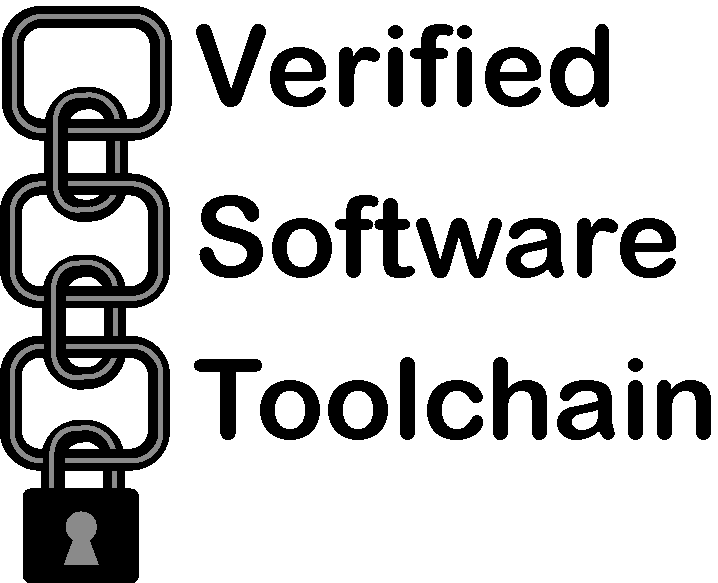
\includegraphics[width=.07\textwidth]{img/chain.png}};


      \draw (0.5,3) node [textstyle, anchor=west, draw=black, thick, minimum width=3cm,minimum height=0.5cm] (ml) {$\Zfield$};
      \draw (0,3) node [anchor=east] (shn) {Mid Level};

      \draw[thick,double, <->, >=implies] (ll.north) -- (ml.south);

      \draw (0.5,4) node [textstyle, anchor=west, draw=black, thick, minimum width=3cm,minimum height=0.5cm] (hl) {$\K$};
      \draw (0,4) node [anchor=east] (shn) {High Level};

      \draw[thick,double, <-, >=implies] (ml.north) -- (hl.south);
    \end{scope}
\end{tikzpicture}

  \caption{Structural construction of the proof}
  \label{tk:ProofStructure}
\end{figure}

\subsection{Correctness specification}

% The soundness is implied by the proof of the following specification.
We show the soundness of TweetNaCl by proving the {\red{equivalence}} of the following
specification. This defines the equivalence between the Clight representation
and a Coq definition of the ladder.

\begin{CoqVST}
Definition crypto_scalarmult_spec :=
DECLARE _crypto_scalarmult_curve25519_tweet
WITH
  v_q: val, v_n: val, v_p: val, c121665:val,
  sh : share,
  q : list val, n : list Z, p : list Z
(*------------------------------------------*)
PRE [ _q OF (tptr tuchar),
     _n OF (tptr tuchar),
     _p OF (tptr tuchar) ]
PROP (writable_share sh;
      Forall (fun x => 0 <= x < 2^8) p;
      Forall (fun x => 0 <= x < 2^8) n;
      Zlength q = 32; Zlength n = 32;
      Zlength p = 32)
LOCAL(temp _q v_q; temp _n v_n; temp _p v_p;
      gvar __121665 c121665)
SEP  (sh [{ v_q }] <<(uch32)-- q;
      sh [{ v_n }] <<(uch32)-- mVI n;
      sh [{ v_p }] <<(uch32)-- mVI p;
      Ews [{ c121665 }] <<(lg16)-- mVI64 c_121665)
(*------------------------------------------*)
POST [ tint ]
PROP (Forall (fun x => 0 <= x < 2^8) (CSM n p);
      Zlength (CSM n p) = 32)
LOCAL(temp ret_temp (Vint Int.zero))
SEP  (sh [{ v_q }] <<(uch32)-- mVI (CSM n p);
      sh [{ v_n }] <<(uch32)-- mVI n;
      sh [{ v_p }] <<(uch32)-- mVI p;
      Ews [{ c121665 }] <<(lg16)-- mVI64 c_121665
\end{CoqVST}

In this specification we state as preconditions:
\begin{itemize}
  \item[] \VSTe{PRE}: \VSTe{_p OF (tptr tuchar)}\\
  The function \texttt{crypto\_scalarmult} takes as input three pointers to
  arrays of unsigned bytes (\VSTe{tptr tuchar}) \VSTe{_p}, \VSTe{_q} and \VSTe{_n}.
  \item[] \VSTe{LOCAL}: \VSTe{temp _p v_p}\\
  Each pointer represent an address \VSTe{v_p},
  \VSTe{v_q} and \VSTe{v_n}.
  \item[] \VSTe{SEP}: \VSTe{sh [{ v_p $\!\!\}\!\!]\!\!\!$ <<(uch32)-- mVI p}\\
  In the memory share \texttt{sh}, the address \VSTe{v_p} points
  to a list of integer values \VSTe{mVI p}.
  \item[] \VSTe{PROP}: \VSTe{Forall (fun x => 0 <= x < 2^8) p}\\
  In order to consider all the possible inputs, we assumed each
  elements of the list \texttt{p} to be bounded by $0$ included and $2^8$
  excluded.
  \item[] \VSTe{PROP}: \VSTe{Zlength p = 32}\\
  We also assumed that the length of the list \texttt{p} is 32. This defines the
  complete representation of \TNaCle{u8[32]}.
\end{itemize}

As Post-condition we have:
\begin{itemize}
  \item[] \VSTe{POST}: \VSTe{tint}\\
  The function \texttt{crypto\_scalarmult} returns an integer.
  \item[] \VSTe{LOCAL}: \VSTe{temp ret_temp (Vint Int.zero)}\\
  The returned integer has value $0$.
  \item[] \VSTe{SEP}: \VSTe{sh [{ v_q $\!\!\}\!\!]\!\!\!$ <<(uch32)-- mVI (CSM n p)}\\
  In the memory share \texttt{sh}, the address \VSTe{v_q} points
  to a list of integer values \VSTe{mVI (CSM n p)}.
  \item[] \VSTe{PROP}: \VSTe{Forall (fun x => 0 <= x < 2^8) (CSM n p)}\\
  \VSTe{PROP}: \VSTe{Zlength (CSM n p) = 32}\\
  We show that the computation for \VSTe{CSM} fits in  \TNaCle{u8[32]}.
\end{itemize}

\todo[inline]{theorem between CSM and Timmy representation here. Eg.}

\begin{lstlisting}[language=CoqD]
Theorem CSM_eq :
  forall (n:list Z) (p:list Z),
  Zlength n = 16 ->
  Zlength p = 16 ->
  Forall (fun x => 0 <= x < 2^8) p ->
  Forall (fun x => 0 <= x < 2^8) n ->
  Z16.lst (CSM n p) = Z16.lst n $\times$ Z16.lst p.
\end{lstlisting}
We proved that \VSTe{crypto_scalarmult} (\VSTe{CSM} in Coq)
computes: $$Q.x \leftarrow N \times P.x$$

where \VSTe{p} represent the x-coordinate of $P$, \VSTe{n} represent the
scalar by which it is be multiplied $N$ (where the bits 1, 2, 5 248, 249, 250
are cleared and bit 6 is set).

% As a result of the excution of \VSTe{crypto_scalarmult}, the value \VSTe{0}
% is returned, \VSTe{p} and \VSTe{n} points to the same locations containing
% the same values \VSTe{pp} and \VSTe{nn}.
% The pointer \VSTe{q} points to the same location, but contain the x coordinate of $Q$.
